\documentclass[a4paper,12pt]{article}
\usepackage[utf8]{inputenc}

\usepackage[a4paper,left=2.5cm,right=2.cm,top=2.5cm,bottom=2.5cm]{geometry}

\usepackage[english]{babel}
\usepackage[babel]{csquotes}

\usepackage[colorlinks=true, allcolors=blue]{hyperref}
\usepackage[all]{hypcap}

\usepackage{graphicx}
\usepackage{subcaption}
\usepackage{booktabs}

\usepackage[style=authoryear, backend=biber, natbib]{biblatex}  
\bibliography{~/Zotero/Bibliothek.bib}

%opening
\title{Interview- and Respondent-level Predictors of Refusal and ``Don't know'' Item Nonresponse in the ESS 9}

\author{Malte Grönemann}

\begin{document}

\begin{titlepage}
\maketitle
\thispagestyle{empty} 

%\centering
\large

Term Paper within the Seminar \\
\textbf{Fundamentals of Survey Design}  \\
FSS 2021 \\
Tobias Gummer\\
University of Mannheim \\
School of Social Sciences

\bigskip

\normalsize

\textbf{Abstract:} In this article, I have a look at interview- and respondent-level predictors of item nonresponse in the ESS Round 9. Using an interviewer fixed-effects negative binomial regression, I confirm most previous findings on the respondent-level: better educated, politically more interested and engaged, more trusting male ethnic majority respondents have lowest rates of item nonresponse. But the interview level is the more interesting one since these predictors actually can help survey researchers to prevent item nonresponse. Besides efforts to ensure respondents understand the survey questions, building a trusting interview situation to ease reluctancy, stimulating motivation and making sure that respondents correctly use showcards are the most promising avenues to reduce item nonresponse. Gender matching and interferences with the interview are not associated with item nonresponse.

\bigskip

\textbf{Keywords:} Item Nonresponse, Data Quality, European Social Survey, F2F, Interview, Fixed-Effects Negative Binomial Regression

\end{titlepage}


\section*{Declaration in Lieu of an Oath}

\setcounter{page}{0}
\thispagestyle{empty} 

„Hiermit versichere ich, dass diese Arbeit von mir persönlich verfasst ist
und dass ich keinerlei fremde Hilfe in Anspruch genommen habe. Ebenso
versichere ich, dass diese Arbeit oder Teile daraus weder von mir selbst
noch von anderen als Leistungsnachweise andernorts eingereicht wurden.
Wörtliche oder sinngemäße Übernahmen aus anderen Schriften und
Veröffentlichungen in gedruckter oder elektronischer Form sind
gekennzeichnet. Sämtliche Sekundärliteratur und sonstige Quellen sind
nachgewiesen und in der Bibliographie aufgeführt. Das Gleiche gilt für
graphische Darstellungen und Bilder sowie für alle Internet-Quellen. Ich
bin ferner damit einverstanden, dass meine Arbeit zum Zwecke eines
Plagiatsabgleichs in elektronischer Form anonymisiert versendet und
gespeichert werden kann. Mir ist bekannt, dass von der Korrektur der
Arbeit abgesehen und die Prüfungsleistung mit „nicht ausreichend“
bewertet werden kann, wenn die Erklärung nicht erteilt wird."
\bigskip

"I hereby declare that the final thesis presented is my own work and that I have not called upon the help of a third party. In addition, I affirm that neither I nor anybody else has submitted this paper or parts of it to obtain credits elsewhere before. I have clearly marked and acknowledged all quotations or references that have been taken from the works of others. All secondary literature  and  other  sources  are  marked  and  listed  in  the  bibliography.  The  same  applies  to  all charts, diagrams and illustrations as well as to all Internet resources. Moreover, I consent to my paper being electronically stored and sent anonymously in order to be checked for plagiarism. I am aware that if this declaration is not made, the thesis may not be graded."

\bigskip

Mannheim, \today

\bigskip
\includegraphics[scale=.1]{/home/malte/Dokumente/Dokumente/Unterschrift_Malte.JPG}
\newpage 

\section{Introduction}

Missing data pose a problem to analysis of survey data because they decrease the effective sample size and can introduce bias to estimations if the causes for missingness are related to the missing item or respondent characteristics \citep{deleeuwPreventionTreatmentItem2003}. Due to these harmful effects of missing data, one objective of survey researchers is to keep their prevalence as low as possible. For this aim, it is important to understand the processes that can lead to missing data.

We can get a first grasp on both the mechanisms causing the missingness and its likely impact on bias by categorising missingness based on their relation to randomness. Missings that are not related to anything are typically called \textit{missing completely at random} and have no impact on bias therefore only decreasing effective sample size. Is the relation between missingness and item not direct but the cause of missingness is related to other characteristics of the respondent, we speak of \textit{missing at random}. MAR additionally has the risk of leading to biased estimates. Even more consequential for bias are data \textit{not missing at random} where the missingness is directly linked to the unknown position to the surveyed topic or unknown value of the item. There is a special case of not missing at random in missings though that is unconsequential because it is controlled: \textit{missing by design}. These are cases, when questions do not apply and are left blank due to filtering procedures \citep[155]{deleeuwPreventionTreatmentItem2003}. The processes generating these types of missing data typically differ. Missings completely at random can be created for example by overlooking a question or a processing error while missings by design is a conscious and deliberate choice in questionnaire design.

In this paper, I focus on missingness due to nonsubstantive answers given by respondents (\textit{item nonresponse}), specifically causes for answer refusals and "Don't know" (DK) answers on the respondent and interview level. Besides unit nonresponse and interview breakoffs, item nonresponse is one of the biggest sources of missing at random and not missing at random. Item nonresponse can also be seen as an indicator for overall data quality since it can indicate satisficing behaviour of the respondent \citep{krosnickResponseStrategiesCoping1991}.

The question-answer process involves multiple steps on behalf of the respondent in the following order: understanding the question, recalling the necessary information from memory, eventually judging information recalled, eventually editing it if the perceived sensitivity or social desirability is high, eventually formating it to fit a response category and finally communicating the response. In all these stages, refusals and DKs can be introduced \citep[pp. 159f]{deleeuwPreventionTreatmentItem2003}.

Refusals and DKs can be attributed to slightly different missingness generating mechanisms though. Refusals are more likely to stem from the editing step when respondents feel an item to be too sensitive. DK is more likely to come about in one of the previous steps if the mental effort to answer a question is too high. But higher mental effort is also related to more refusals \citep{shoemakerItemNonresponseDistinguishing2002}. DK can therefore be seen as a strategy of \textit{(strong) satisficing}, giving a satisfactory answer instead of bothering to actually think about a question in depth (\textit{optimising}) \citep[219]{krosnickResponseStrategiesCoping1991}. Consequentially, DK answers are more likely to be missing at random and refusals are more likely to be not missing at random.

Although the respondent is the one giving the answers in the end, the causes and amplifiers of item nonresponse are manifold and not only vary by which step of the question-answer process they influence \citep{holbrookImpactQuestionRespondent2006} on but also their hierarchical level. This starts with country and survey characteristics and spanning interviewer effects, respondent characteristics, the interview situation, the questionnaire and ends at the individual item. I proceed with a short review of influencing factors of item nonresponse ordered by their level.

\bigskip

\textbf{Country}:
Considerable country-level differences have been observed but there are no convincing explanations for these differences to date. \citet{meitingerPowerCultureItem2020} study how cultural and socio-economic characteristics influence item nonresponse but only uncertainty avoidance turned out to significantly increase levels of item nonresponse. Other country-level variables like individualisation and inequality had the expected direction though. Norms vary geographically that define how sensitive a topic is and what socially acceptable answers are (see below). Some variance between countries stems from composition effects \citep{kochItemNonresponseEuropean2009}.

\textbf{Survey}:
Survey characteristics like mode, topic and incentives as well as instructions to interviewers on refusal conversion, contacting etc. could influence the composition of realised interviews and therefore indirectly have an effect on item nonresponse. Parts of the differences in item nonresponse rates between mail and web modes can be attributed to different demographic compositions of the obtained samples \citep{messerDeterminantsItemNonresponse2012} and refusal conversions often show higher item nonresponse \citep{yanRelationUnitNonresponse2010}. Survey mode also influences the design possibilities of the questionnaire (see below) and the likelihood of respondents or interviewers overlooking questions or processing errors.

\textbf{Interviewer}:
There is often substantial variance in item nonresponse between interviewers. But associations between item nonresponse and interviewer characteristics are not clear cut (e.g. \cite{pickeryImpactRespondentInterviewer1998, pickeryExplorationQuestionCharacteristics2001, silberEffectsQuestionRespondent2021}). But there are hints that older interviewers obtain more item nonresponse and interviewer training can reduce nonresponse \citep{silberEffectsQuestionRespondent2021}.

Explicitly coded refusals or ``Don't know'' answers can also be accidentally misreported by the interviewer or even deliberately changed from a substantial answer to shorten on follow-up questions \citep[165]{deleeuwPreventionTreatmentItem2003}.

\textbf{Respondent}:
The question-answer process requires motivation on behalf of the respondent to cooperate and the mental ability to perform the necessary tasks to get to an answer. Differences in mental ability have quite frequently be related to item nonresponse and are a reasonable explanation for the often observed higher item nonresponse rates of elderly and lower educated respondents \citep{pickeryImpactRespondentInterviewer1998, deleeuwPreventionTreatmentItem2003, messerDeterminantsItemNonresponse2012, silberEffectsQuestionRespondent2021}. This reasoning is supported by correlations between item nonresponse and direct measures of intelligence but also to levels of conscentiousness \citep{hedengrenDogThatDidn2012} and to measures of physical and mental health \citep{colsherDataQualityAge1989}. Women and ethnic minorities are also often found to have more item nonresponse \citep{pickeryImpactRespondentInterviewer1998, kupekDeterminantsItemNonresponse1998}. For the latter, this might be connected to the finding that lower literacy and language ability increases item nonresponse \citep{kupekDeterminantsItemNonresponse1998}. \citet{meitingerPowerCultureItem2020} interpret these findings in a social marginalisation and power perspective: item nonresponse reflects broader social inequalities in abilities and access to information.
Respondents that are more interested in the topic of the survey have found to have lower item nonresponse likely due to their higher motivation \citep{kochItemNonresponseEuropean2009, silberEffectsQuestionRespondent2021}. Reluctancy to answer and overall skepticism towards surveys and science, privacy concerns, generalised mistrust are personality traits that result in more nonresponse \citep{silberEffectsQuestionRespondent2021}. These are also related to unit nonresponse. The idea of a trade-off between unit and item nonresponse is summarised by \citet{yanRelationUnitNonresponse2010} in their \textit{response continuum model}.

\textbf{Interview}:
Interview characteristics and interactions between interviewer and respondent characteristics have gained a little attention in past research. \citet{vercruyssenEffectSociodemographicMis2017} find less item nonresponse when matching age of interviewers and respondents in the ESS in Belgium while gender matching reduces item nonresponse for males and increases it for females. Matching education has no significant effect after controlling for respondents education. \citet{silberEffectsQuestionRespondent2021} obtain similar results in Germany. Gender matching is also less important while age and education matching are potent predictors of item nonresponse in a sex survey in Taiwan \citep{tuSocialDistanceRespondent2007}.
 
 Other people present during the interview resulted in higher item nonresponse sometimes \citep{kupekDeterminantsItemNonresponse1998} but not always \citep{tuSocialDistanceRespondent2007, silberEffectsQuestionRespondent2021}. Respondent cooperation as perceived by the interviewer also predicts lower item nonresponse \citep{tuSocialDistanceRespondent2007} but again with exeptions \citep{silberEffectsQuestionRespondent2021}.
 
\textbf{Questionnaire}:
 Questionnaire design choices like wether DK was explicitly offered but also the complexity of a questionnaire with changes in response categories, routing and filtering are associated with higher nonresponse \citep{messerDeterminantsItemNonresponse2012} likely due to higher likelihoods of mistakes by respondents or interviewers and processing errors. Page layout and progress bars in web surveys have also been discussed to influence item nonresponse \citep{peytchevWebSurveyDesign2006, yanShouldStayShould2011, sarrafSurveyPageLength2014}. Also, a long questionnaire might fatigue respondents giving more nonsubstantial answers later on.
 
\textbf{Question}:
The previous point directly relates to a questions position within the questionnaire. But besides fatigue later on, there might also be a learning effect reducing item nonresponse over time \citep{holbrookInterviewerErrorsHelp2016, olsonEffectsRespondentQuestion2019}.
Item non-response varies between questions with more sensitive questions typically having higher item nonresponse. Most prominently, this affects questions on income \citep{yanTrendsIncomeNonresponse2010} and sexual behaviour \citep{kupekDeterminantsItemNonresponse1998} but \citet{olsonEffectsRespondentQuestion2019} suggests that eventually, a nonsubstantial answer might be even more telling resulting in lower levels of nonresponse. More difficult or unclear questions typically have higher item nonresponse as well but question length of itself is not \citep{holbrookImpactQuestionRespondent2006, messerDeterminantsItemNonresponse2012, holbrookInterviewerErrorsHelp2016, olsonEffectsRespondentQuestion2019}. Consequentially, attitudinal and behavioural questions often produce more item nonresponse than demographic questions \citep{olsonEffectsRespondentQuestion2019, silberEffectsQuestionRespondent2021}. And design decisions on the question level infuence the cognitive effort needed to provide a substantial answer as well: open-ended questions, being allowed to select multiple options, more response categories and ordering categories are associated with higher nonresponse due to difficulty and burden \citep{holbrookImpactQuestionRespondent2006, holbrookInterviewerErrorsHelp2016, olsonEffectsRespondentQuestion2019, silberEffectsQuestionRespondent2021}. \citet{holbrookInterviewerErrorsHelp2016} found that questions using showcards had more problems although this is likely not because of the showcards but because they are only used with more difficult questions. The question level is one of the best understood levels and constitutes the largest part of the variance. This highlights the importance of the single question for overall data quality \citep{olsonEffectsRespondentQuestion2019}.

\bigskip

To improve data quality, there are a few things we have some control over, mainly considering the interview situation, the interviewers and the survey characteristics including questionnaire and question design. It is therefore reasonable to have a special interest in these to improve data quality. Therefore, the high proportion of explained variance on the question level is good news for survey research. But unfortunately, all of the other manipulatable levels are underresearched. This is most likely due to limited availability of data on the respective concepts.

This article tries to shed some more light on the interview level using paradata and interviewer observations. But since we cannot statistically separate the interview and the unchangeable respondent characteristics, I control for them as well.


\section{Data and Methods}

I analyse item nonresponse in the \textit{European Social Survey (ESS)} Round 9 (version 3.1) \citep{essericEuropeanSocialSurvey2019}. My dependent variables are the number of refusals and DKs as well as a sum of both over all questions that are not affected by routing. 

Since our dependent variables are count data and show overdispersion, I opted for a negative binomial regression (NB II) with interviewer fixed effects \citep{allisonFixedEffectsNegativeBinomial2002}. Country differences are absorbed by the interviewer fixed effects as well. I opted for standard errors clustered by interviewer. Since the population of interest in this case are the realised interviews and not societies, no weighting is applied. 

Only complete cases are analysed, reducing the sample size from 49,519 to 41,205. The large drop in sample size largely originates from the age of the interviewer and the interview duration, not from item nonresponse on behalf of the respondents. Time stamps have been troublesome in some countries due to errors in the CAPI instrument and Romania used the wrong format for interviewer age \citep{essericESS9CodebookEd2021}. Additionally, some interview durations are suspiciously long, so I top-coded the length of the interview to 3 hours.

The respondent-level variables are from the original questionnaire while the interview-level variables are either calculated from paradata or are interviewer observations recorded after the interview in the interviewer questionnaire. Most predictors are measured on a 5-point Likert scale. If they are not, they are either recoded to make relative effect size comparisons or their scale is mentioned in brackets in the results section. Categorical predictors (gender, group memberships, interview interference, interview language, gender and age matching) are included as dummy variables.

The analyses are carried out in \textit{R} \citep{rcoreteamLanguageEnvironmentStatistical2021} using the \textit{Tidyverse} packages \citep{wickhamWelcomeTidyverse2019} for data handling and graphics and the \textit{fixest} package \citep{bergeEfficientEstimationMaximum2018} to estimate the regression. The code is available \href{https://github.com/maltegroenemann/inr_ess9}{here}.


\section{Results}

\begin{figure}
\caption{Results of the Fixed-Effects Negative Binomial Regression}
 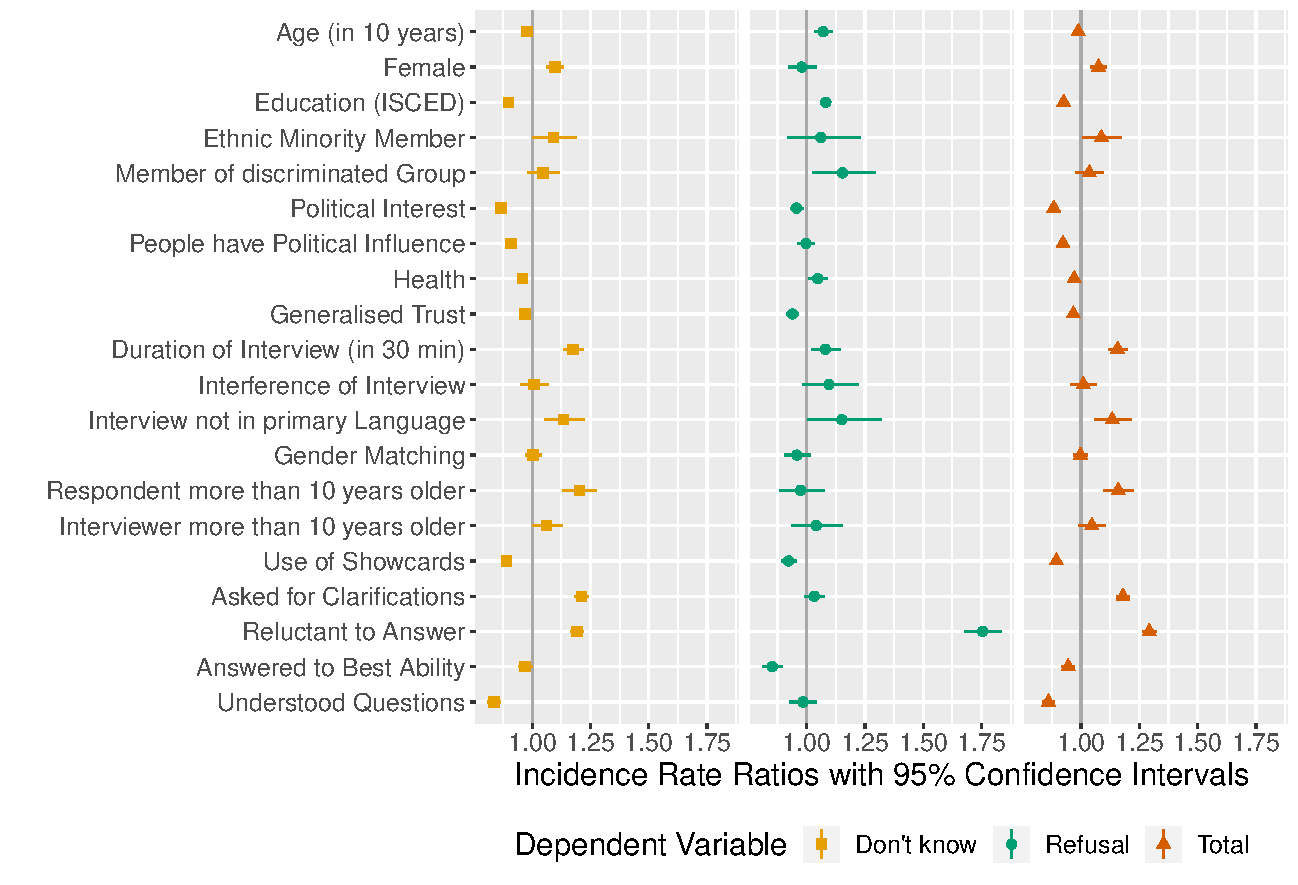
\includegraphics[width=.99\textwidth]{results.pdf}
 \label{results}
\end{figure}


Figure \ref{results} shows the regression results for the three dependent variables. Starting with the respondent level, older people are associated with slightly less DKs but more refusals leading to no significant relation between age and total item nonresponse. Women show slightly more DKs than men. Higher education is associated with less DKs but more refusals. Members of ethnic minorities are associated with more DKs while members of discriminated groups have more refusals on average. The more respondents are interested in politics, the fewer DKs and refusals they give in this mainly political survey. The more respondents believe that the political system allows them to have influence, the fewer DKs. A better health is associated with fewer DKs but more refusals. And finally, the more respondents trust generalised others, the fewer DKs and refusals.

At the interview level, a longer interview is associated with more of both types of nonresponse. But other people present or interfering during the interview shows no relation to either. If the interview is conducted in a language different from the one primarily spoken at the respondents home, more DKs and refusals are predicted. Matching genders of the interviewer and the respondent has no relation to item nonresponse and remains so when interacted with respondents gender (not shown). More DKs are predicted when the respondent is more than ten years older than the interviewer. The extent of the respondents accurately using the showcards is negatively related to both types of nonresponse. The respondent more often asking for clarifications is associated with more DK nonresponse. The interviewer perceiving the respondent to be reluctant increases both DKs and especially refusals. The more repondents tried to answer to the best of their abilities, the fewer nonresponse and the better the respondents understands the questions, the fewer DKs.

If not mentioned otherwise, the relations concerning the total amount of item nonresponse mirror the relation with DK. This is hardly surprising since DK is much more frequent. There are in total 176,490 DKs (on average 3.5 per respondent) over all variables unaffected by routing but only 41,821 refusals (0.8 per respondent).

The results from Figure \ref{results} are displayed in a regression table in the appendix as well.


\section{Conclusion}

This article set out to improve our understanding of item nonresponse, a typical indicator of data quality, focussing on the interview- and the respondent-level. 

Compared to previous results and common explanations for repondent-level variables, most results are in line with them: better educated, politically more interested and engaged, more trusting male ethnic majority respondents have lowest rates of item nonresponse. But there are some surprising findings as well: education differs in its effect by type of nonresponse. This might be due to them being more able and knowing but at the the same time more conscious about privacy. Privacy concerns might also be hightened for members of discriminated groups resulting in more refusals. Health did also differ in its effect by type of nonresponse. Age on the other hand has not the expected effect though. But this is likely due to controlling for measures of cognitive ability. This holds true for all variables though, the effects are all conditional on the other independent variables. Understanding their separate effects and potential mediations is beyond the scope of the article though.

The more interesting results however are the ones on the interview level because they can actually be changed and therefore be considered in the design of future surveys. Interference of the interview and matching respondents and interviewers gender has no effect at least in this attitude survey. With more sensitive topics, this might be different though. A longer interview and asking for many clarifications are associated with more item nonresponse but are likely just resulting from the common cause of understanding difficulties. Taken together with the interviewers assessment of the respondents understanding of the questions, this again highlights the importance of question design for data quality. One possibility to improve understanding is to conduct the interview in the respondents primary language but it is a trade with costs and comparability. Increasing respondents motivation, the underlying concept of whether respondents answered to their best ability, also could improve data quality. But besides understanding of the questions, the effects largest in magnitude are respondents reluctancy (especially considering refusals which are likely to be not missing at random) and their use of showcards. Building a trusting interview situation and making sure that respondents correctly use the showcards are the most promising avenues to reduce item nonresponse.

But as with all cross-sectional analyses, these coefficients merely represent associations, not causal effects. Separating the causal effects using survey experiments as well as improving on our understanding of mediating and confounding relations between these variables are left for further research. Especially since most interview-level predictors are subjective assessments by the interviewers and therefore endogenous \citep[8]{silberEffectsQuestionRespondent2021}. And there might still be variables and concepts on both levels that have been omitted due to inavailability. Examples are attitudes on personal privacy, trust in science (coming in ESS10) as well as better measures of motivation and commitment.


\printbibliography

\section*{Appendix: Table of the Regression Results}
\small
\begin{tabular}{lccc}
\tabularnewline\midrule\midrule
Dependent Variables:&DK&Refusals&Total\\
Model:&(1) & (2) & (3)\\
\midrule \emph{Variables}&   &   &  \\
`Age(in10years)` & -0.022$^{**}$ (0.010) & 0.068$^{***}$ (0.018) & -0.012 (0.010)\\
Female & 0.093$^{***}$ (0.018) & -0.021 (0.031) & 0.072$^{***}$ (0.016)\\
`Education(ISCED)` & -0.107$^{***}$ (0.006) & 0.079$^{***}$ (0.009) & -0.078$^{***}$ (0.005)\\
`EthnicMinorityMember` & 0.088$^{**}$ (0.043) & 0.059 (0.075) & 0.084$^{**}$ (0.039)\\
`MemberofdiscriminatedGroup` & 0.045 (0.033) & 0.143$^{**}$ (0.059) & 0.035 (0.030)\\
`PoliticalInterest` & -0.143$^{***}$ (0.008) & -0.044$^{***}$ (0.015) & -0.125$^{***}$ (0.008)\\
`PeoplehavePoliticalInfluence` & -0.095$^{***}$ (0.011) & -0.003 (0.019) & -0.081$^{***}$ (0.010)\\
Health & -0.043$^{***}$ (0.010) & 0.046$^{**}$ (0.020) & -0.030$^{***}$ (0.010)\\
`GeneralisedTrust` & -0.032$^{***}$ (0.008) & -0.062$^{***}$ (0.014) & -0.034$^{***}$ (0.007)\\
`DurationofInterview(in30min)` & 0.161$^{***}$ (0.019) & 0.077$^{***}$ (0.029) & 0.146$^{***}$ (0.018)\\
`InterferenceofInterview` & 0.007 (0.030) & 0.091$^{*}$ (0.055) & 0.009 (0.028)\\
`InterviewnotinprimaryLanguage` & 0.127$^{***}$ (0.038) & 0.141$^{**}$ (0.070) & 0.126$^{***}$ (0.036)\\
`GenderMatching` & 0.004 (0.017) & -0.043 (0.030) & -0.002 (0.016)\\
`Respondentmorethan10yearsolder` & 0.184$^{***}$ (0.031) & -0.026 (0.050) & 0.148$^{***}$ (0.029)\\
`Interviewermorethan10yearsolder` & 0.060$^{*}$ (0.031) & 0.040 (0.053) & 0.045 (0.029)\\
`UseofShowcards` & -0.115$^{***}$ (0.011) & -0.080$^{***}$ (0.018) & -0.112$^{***}$ (0.010)\\
`AskedforClarifications` & 0.191$^{***}$ (0.013) & 0.032 (0.021) & 0.165$^{***}$ (0.011)\\
`ReluctanttoAnswer` & 0.175$^{***}$ (0.012) & 0.562$^{***}$ (0.023) & 0.257$^{***}$ (0.012)\\
`AnsweredtoBestAbility` & -0.030$^{*}$ (0.016) & -0.160$^{***}$ (0.026) & -0.057$^{***}$ (0.015)\\
`UnderstoodQuestions` & -0.178$^{***}$ (0.017) & -0.016 (0.030) & -0.151$^{***}$ (0.016)\\
\midrule \emph{Fixed-effects}&   &   &  \\
Interviewer & Yes & Yes & Yes\\
\midrule \emph{Fit statistics}&  & & \\
Observations & 39,984&32,998&40,281\\
Squared Correlation & 0.37252&0.21577&0.37939\\
Pseudo R$^2$ & 0.12134&0.18078&0.12375\\
BIC & 176,801.4&80,964.8&190,729.0\\
Over-dispersion & 0.94260&0.79857&1.0881\\
\midrule\midrule\multicolumn{4}{l}{\emph{One-way (Interviewer) standard-errors in parentheses}}\\
\multicolumn{4}{l}{\emph{Signif. Codes: ***: 0.01, **: 0.05, *: 0.1}}\\
\end{tabular}



\end{document}
